% Provenance (never printed): cycle 2 "Questionner le monde de la matiere"
% (solid materials, observing and sorting) and cycle 3 theme 4 (local geology,
% rocks for building); see sources/book1/PROVENANCE.md. Book 1, grade 3, ch. 1.
\chapter{Stones, Pebbles and Sand}\label{ch:g3:stones-pebbles-sand}

Tom is on holiday by a \omterm{def:g1:landscapes-around-us:water}{river}. On the \omterm{def:g3:stones-pebbles-sand:pebble}{gravel} bank, where the water is
shallow, he picks up a \omterm{def:g3:stones-pebbles-sand:pebble}{pebble}. It is smooth and round, almost like an egg,
and it fits in his hand. Last week, walking with his parents on a \omterm{def:g1:landscapes-around-us:landform}{mountain}
path high up the same \omterm{def:g1:landscapes-around-us:landform}{valley}, he saw stones of the same colour lying under
a rocky slope --- but those stones were sharp, with edges and corners.

How did a sharp stone from the \omterm{def:g1:landscapes-around-us:landform}{mountain} become a smooth, round \omterm{def:g3:stones-pebbles-sand:pebble}{pebble} down
in the \omterm{def:g1:landscapes-around-us:landform}{valley}? To find out, let us start with the \omterm{def:g3:stones-pebbles-sand:rock}{rock} itself.

\begin{omfigure}
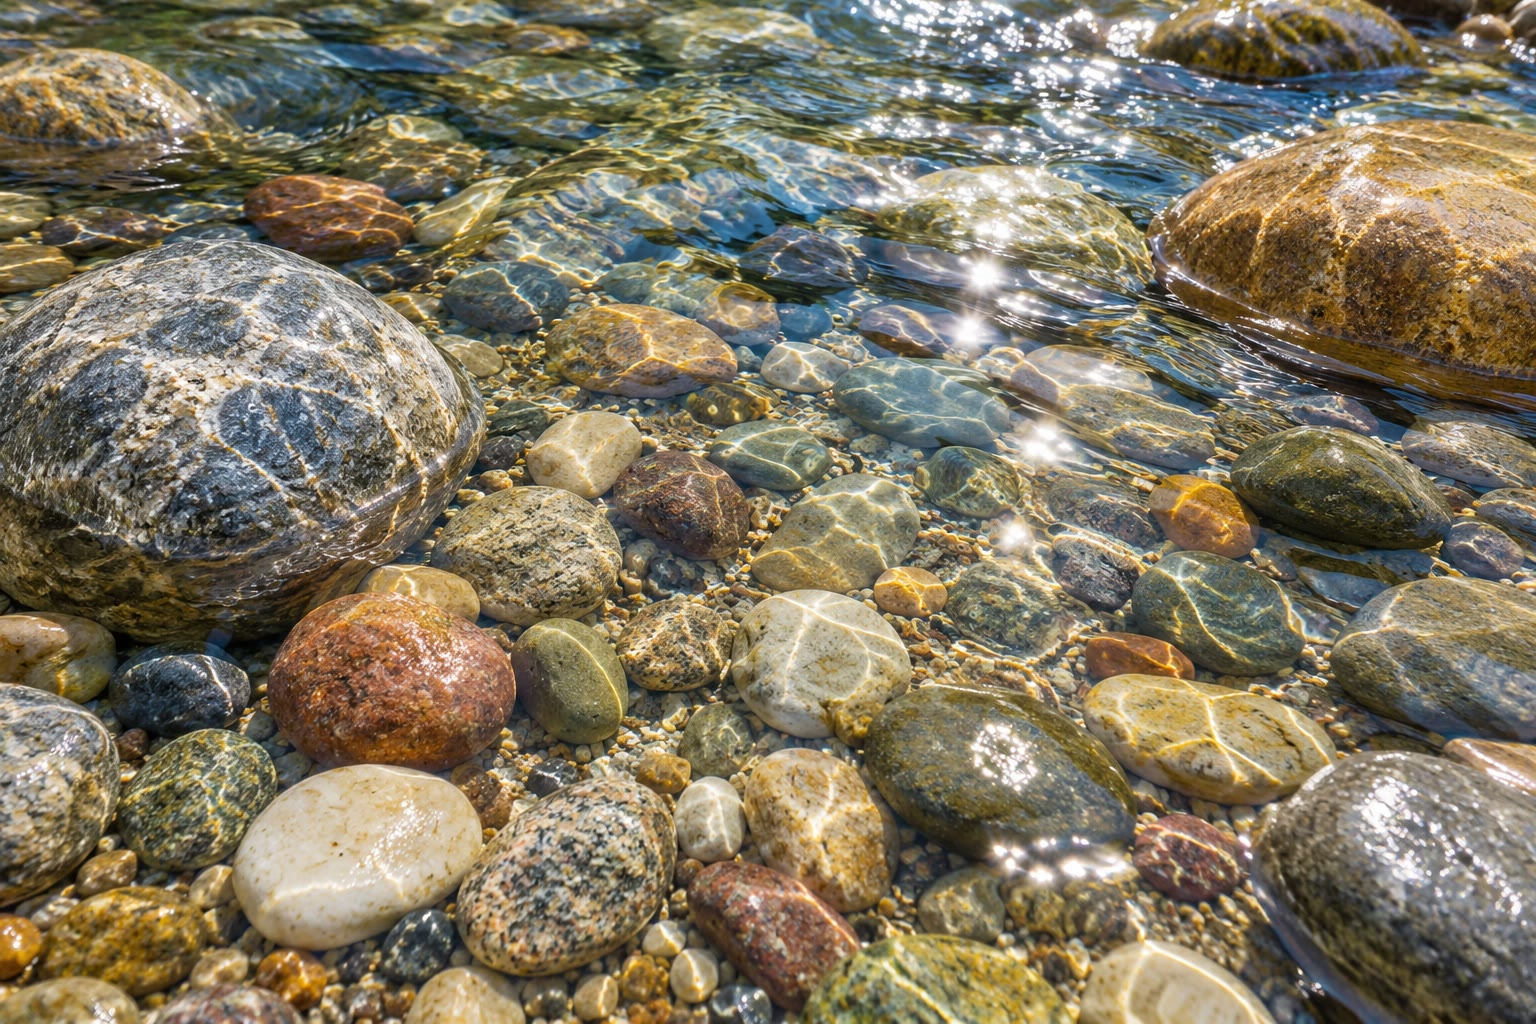
\includegraphics[width=0.62\linewidth]{images/book1/ai/g3-stream-pebbles.jpg}

{\small Round \omterm{def:g3:stones-pebbles-sand:pebble}{pebbles} under the clear water of a stream.}
\end{omfigure}

\begin{recall}
In a \omterm{def:g1:landscapes-around-us:landscape}{landscape} there are \omterm{def:g1:landscapes-around-us:landform}{mountains}, \omterm{def:g1:landscapes-around-us:landform}{hills}, \omterm{def:g1:landscapes-around-us:landform}{valleys} and \omterm{def:g1:landscapes-around-us:landform}{plains}, and \omterm{def:g1:landscapes-around-us:water}{rivers}
that flow from the high land down to the \omterm{def:g2:water-on-earth:ocean}{sea}
(\cref{ch:g1:landscapes-around-us}). The top layer of the ground, where
plants grow, is the soil: the biology books tell how living things make
it.
\end{recall}

\section{Rock: the hard ground under our feet}

Dig a deep hole in a garden. First you find dark, soft soil with roots in
it. Below, the soil becomes lighter and stonier. And if you could dig deep
enough, you would always reach something hard that a spade cannot cut:
\omterm{def:g3:stones-pebbles-sand:rock}{rock}.

\begin{definition}[Rock and bedrock]\label{def:g3:stones-pebbles-sand:rock}
A \emph{rock}\index{rock} is a hard, natural material that the solid Earth
is made of. The \emph{bedrock}\index{bedrock} is the solid rock that lies
under the soil everywhere on the land, and under the \omterm{def:g3:stones-pebbles-sand:sand}{sand} and the \omterm{def:g3:stones-pebbles-sand:sand}{mud} of
the \omterm{def:g2:water-on-earth:ocean}{sea} floor.
\end{definition}

In most places the \omterm{def:g3:stones-pebbles-sand:rock}{bedrock} is hidden by the soil, the grass and the trees.
We see it where there is no soil to cover it: in the steep sides of
\omterm{def:g1:landscapes-around-us:landform}{mountains}, in cliffs by the \omterm{def:g2:water-on-earth:ocean}{sea}, and along roads that have been cut through
a \omterm{def:g1:landscapes-around-us:landform}{hill}.

\begin{omfigure}
\begin{tikzpicture}[x=1cm, y=1cm, font=\small]
  % bedrock
  \fill[omLithGranite!60] (0,0) rectangle (11,2.2);
  \foreach \x/\y in {0.6/0.5, 1.8/1.4, 3.1/0.7, 4.4/1.6, 5.6/0.4, 6.9/1.2, 8.3/0.6, 9.6/1.5, 10.3/0.4}
    \draw[black!40, line width=0.4pt] (\x,\y) -- ++(0.5,0.25);
  % soil (thick on the left, missing on the steep right)
  \fill[brown!55] (0,2.2) -- (0,3.4) .. controls (2,3.5) and (4,3.4) .. (5.6,3.2) -- (6.4,2.9) -- (6.4,2.2) -- cycle;
  \fill[brown!30] (0,2.2) rectangle (6.4,2.65);
  % rock showing on the right: a hill side with no soil
  \fill[omLithGranite!60] (6.4,2.2) -- (6.4,2.9) -- (7.6,3.9) -- (8.8,4.3) -- (11,4.3) -- (11,2.2) -- cycle;
  \draw[black!60] (0,3.4) .. controls (2,3.5) and (4,3.4) .. (5.6,3.2) -- (6.4,2.9) -- (7.6,3.9) -- (8.8,4.3) -- (11,4.3);
  % grass and roots
  \foreach \x in {0.3,0.8,...,5.3}
    \draw[green!50!black, line width=0.6pt] (\x,{3.4-0.04*\x}) -- ++(0.05,0.18);
  \foreach \x in {1.2,3.4,4.9}
    \draw[brown!80!black, line width=0.5pt] (\x,3.3) -- ++(-0.1,-0.5) -- ++(0.15,-0.3);
  % labels
  \node[anchor=west] at (11.2,3.6) {rock seen at};
  \node[anchor=west] at (11.2,3.2) {the surface};
  \draw[black!60] (11.15,3.4) -- (9.6,4.15);
  \node[anchor=east] at (-0.2,2.9) {soil};
  \draw[black!60] (-0.15,2.9) -- (0.6,2.9);
  \node[anchor=west] at (11.2,1.1) {bedrock};
  \draw[black!60] (11.15,1.1) -- (10.6,1.1);
\end{tikzpicture}

{\small A cut through the ground. Under the soil there is always the solid
\omterm{def:g3:stones-pebbles-sand:rock}{bedrock}. On the steep \omterm{def:g1:landscapes-around-us:landform}{hill} side, on the right, the soil is missing and the
\omterm{def:g3:stones-pebbles-sand:rock}{rock} shows at the surface.}
\label{fig:g3:stones-pebbles-sand:ground}
\end{omfigure}

\section{From rock to pebbles}

\omterm{def:g3:stones-pebbles-sand:rock}{Rock} is hard, but it does not last for ever. In winter, water gets into
the cracks of a \omterm{def:g3:stones-pebbles-sand:rock}{rock}, freezes and swells, and pushes the cracks wider.
Roots grow into cracks too. Little by little, pieces break off and fall:
that is where the sharp stones under the \omterm{def:g1:landscapes-around-us:landform}{mountain} slopes come from.

When a sharp stone falls into a \omterm{def:g1:landscapes-around-us:landform}{mountain} stream, the water rolls it along
the bottom, knocks it against other stones, and drags it over \omterm{def:g3:stones-pebbles-sand:sand}{sand}. Its
corners are the first to wear away. The farther it travels, the rounder and
smoother it becomes. By the time it reaches the lower \omterm{def:g1:landscapes-around-us:landform}{valley}, it has
become a \omterm{def:g3:stones-pebbles-sand:pebble}{pebble}.

\begin{definition}[Pebble and gravel]\label{def:g3:stones-pebbles-sand:pebble}
A \emph{pebble}\index{pebble} is a small piece of \omterm{def:g3:stones-pebbles-sand:rock}{rock} that has been
rounded and smoothed by water rolling it along, in a \omterm{def:g1:landscapes-around-us:water}{river} or on a beach.
\emph{Gravel}\index{gravel} is a mass of small stones and pebbles lying
together, with grains bigger than grains of \omterm{def:g3:stones-pebbles-sand:sand}{sand}.
\end{definition}

\begin{omfigure}
\begin{tikzpicture}[x=1cm, y=1cm, font=\small]
  \draw[ocBlue!70!black, line width=1.2pt, -{Stealth[length=3mm]}] (0,0) -- (12.2,0);
  \node[below, font=\scriptsize] at (6.1,-0.15) {the stream carries the stone downhill, a little farther every flood};
  \foreach \x/\shape/\t in {
     0.8/{(-0.55,-0.1) -- (-0.2,0.5) -- (0.35,0.55) -- (0.6,0.05) -- (0.3,-0.45) -- (-0.35,-0.5) -- cycle}/fallen from the rock,
     4.0/{(-0.5,-0.1) [rounded corners=4pt] -- (-0.2,0.45) -- (0.3,0.5) -- (0.55,0.05) -- (0.3,-0.4) -- (-0.35,-0.45) -- cycle}/corners worn,
     7.2/{(-0.45,-0.05) [rounded corners=8pt] -- (-0.15,0.42) -- (0.3,0.45) -- (0.5,0.05) -- (0.3,-0.35) -- (-0.3,-0.4) -- cycle}/rounder and smaller,
     10.4/{(0,0) ellipse (0.45 and 0.3)}/a smooth pebble} {
    \begin{scope}[shift={(\x,1.1)}]
      \fill[omLithGranite!80, draw=black!70] \shape;
    \end{scope}
    \node[font=\scriptsize] at (\x,0.35) {\t};
  }
\end{tikzpicture}

{\small The journey of a stone in a \omterm{def:g1:landscapes-around-us:water}{river}: sharp when it falls from the
\omterm{def:g3:stones-pebbles-sand:rock}{rock}, round and smooth after a long ride downstream.}
\label{fig:g3:stones-pebbles-sand:journey}
\end{omfigure}

\begin{remark}[Reading the shape of a stone]\label{rem:g3:stones-pebbles-sand:shape}
The shape of a stone tells us its story. A sharp stone has not travelled
far from the \omterm{def:g3:stones-pebbles-sand:rock}{rock} it broke from. A round, smooth \omterm{def:g3:stones-pebbles-sand:pebble}{pebble} has been rolled for
a long time by water, in a \omterm{def:g1:landscapes-around-us:water}{river} or by the waves of the \omterm{def:g2:water-on-earth:ocean}{sea}.
\end{remark}

\section{Sand and mud}

The stones and \omterm{def:g3:stones-pebbles-sand:pebble}{pebbles} that bump into one another also chip off tiny
pieces. Over a very long time, these tiny pieces become \omterm{def:g3:stones-pebbles-sand:sand}{sand}. Look at \omterm{def:g3:stones-pebbles-sand:sand}{sand}
through a magnifying glass: each grain is a little piece of \omterm{def:g3:stones-pebbles-sand:rock}{rock}, or of a
shell, often rounded too.

\begin{definition}[Sand and mud]\label{def:g3:stones-pebbles-sand:sand}
% ledger: usgs:wentworth
\emph{Sand}\index{sand} is made of loose grains of broken \omterm{def:g3:stones-pebbles-sand:rock}{rock} smaller than
2 millimetres across: we can still see each grain. \emph{Mud}\index{mud} is
made of grains so small that we cannot see them one by one; wet, it is
soft and sticky.
\end{definition}

Geologists sort broken pieces of \omterm{def:g3:stones-pebbles-sand:rock}{rock} by size, from the biggest to the
smallest: boulders, \omterm{def:g3:stones-pebbles-sand:pebble}{pebbles} and \omterm{def:g3:stones-pebbles-sand:pebble}{gravel}, \omterm{def:g3:stones-pebbles-sand:sand}{sand}, and \omterm{def:g3:stones-pebbles-sand:sand}{mud}.

\begin{omfigure}
\begin{tikzpicture}[x=1mm, y=1mm, font=\small]
  % true size: 1 unit = 1 mm
  \draw[black!40] (0,-14) -- (150,-14);
  \foreach \x in {0,10,...,150} \draw[black!40] (\x,-14) -- (\x,-12.5);
  \foreach \x in {0,50,100,150} \node[font=\scriptsize, below] at (\x,-14.5) {\pgfmathparse{int(\x/10)}\pgfmathresult\,cm};
  % mud: too small
  \node[font=\scriptsize, align=center] at (6,14) {mud};
  \fill[brown!60] (6,0) circle (0.05);
  \node[font=\scriptsize, align=center] at (6,4.5) {grains too\\small to see};
  % sand grains: up to 2 mm
  \node[font=\scriptsize] at (28,14) {sand};
  \foreach \x/\r in {22/0.3, 25/0.5, 28/0.75, 32/1.0}
    \fill[yellow!60!brown, draw=black!50, line width=0.2pt] (\x,0) circle (\r);
  \node[font=\scriptsize, align=center] at (28,5) {smaller than\\2 millimetres};
  % gravel and pebbles
  \node[font=\scriptsize] at (78,22) {gravel and pebbles};
  \fill[omLithGranite!80, draw=black!60] (52,0) ellipse (2 and 1.5);
  \fill[black!25, draw=black!60] (62,0) ellipse (4 and 3);
  \fill[omLithGranite!80, draw=black!60] (78,0) ellipse (8 and 6);
  \fill[black!30, draw=black!60] (104,0) ellipse (15 and 10);
  % boulder: off scale
  \node[font=\scriptsize] at (138,22) {boulder};
  \fill[black!20, draw=black!60] (128,-10) .. controls (127,8) and (135,16) .. (142,15) .. controls (150,14) and (152,4) .. (149,-10) -- cycle;
  \node[font=\scriptsize, align=center, fill=white, fill opacity=0.7, text opacity=1, inner sep=1pt] at (139,4) {drawn much\\too small};
\end{tikzpicture}

{\small Grains of broken \omterm{def:g3:stones-pebbles-sand:rock}{rock} from the smallest to the biggest. \omterm{def:g3:stones-pebbles-sand:sand}{Mud}, \omterm{def:g3:stones-pebbles-sand:sand}{sand},
\omterm{def:g3:stones-pebbles-sand:pebble}{gravel} and \omterm{def:g3:stones-pebbles-sand:pebble}{pebbles} are drawn at their real size: compare with a ruler. A
boulder can be as big as a chair, or as a house.}
\label{fig:g3:stones-pebbles-sand:sizes}
\end{omfigure}

\begin{omfigure}
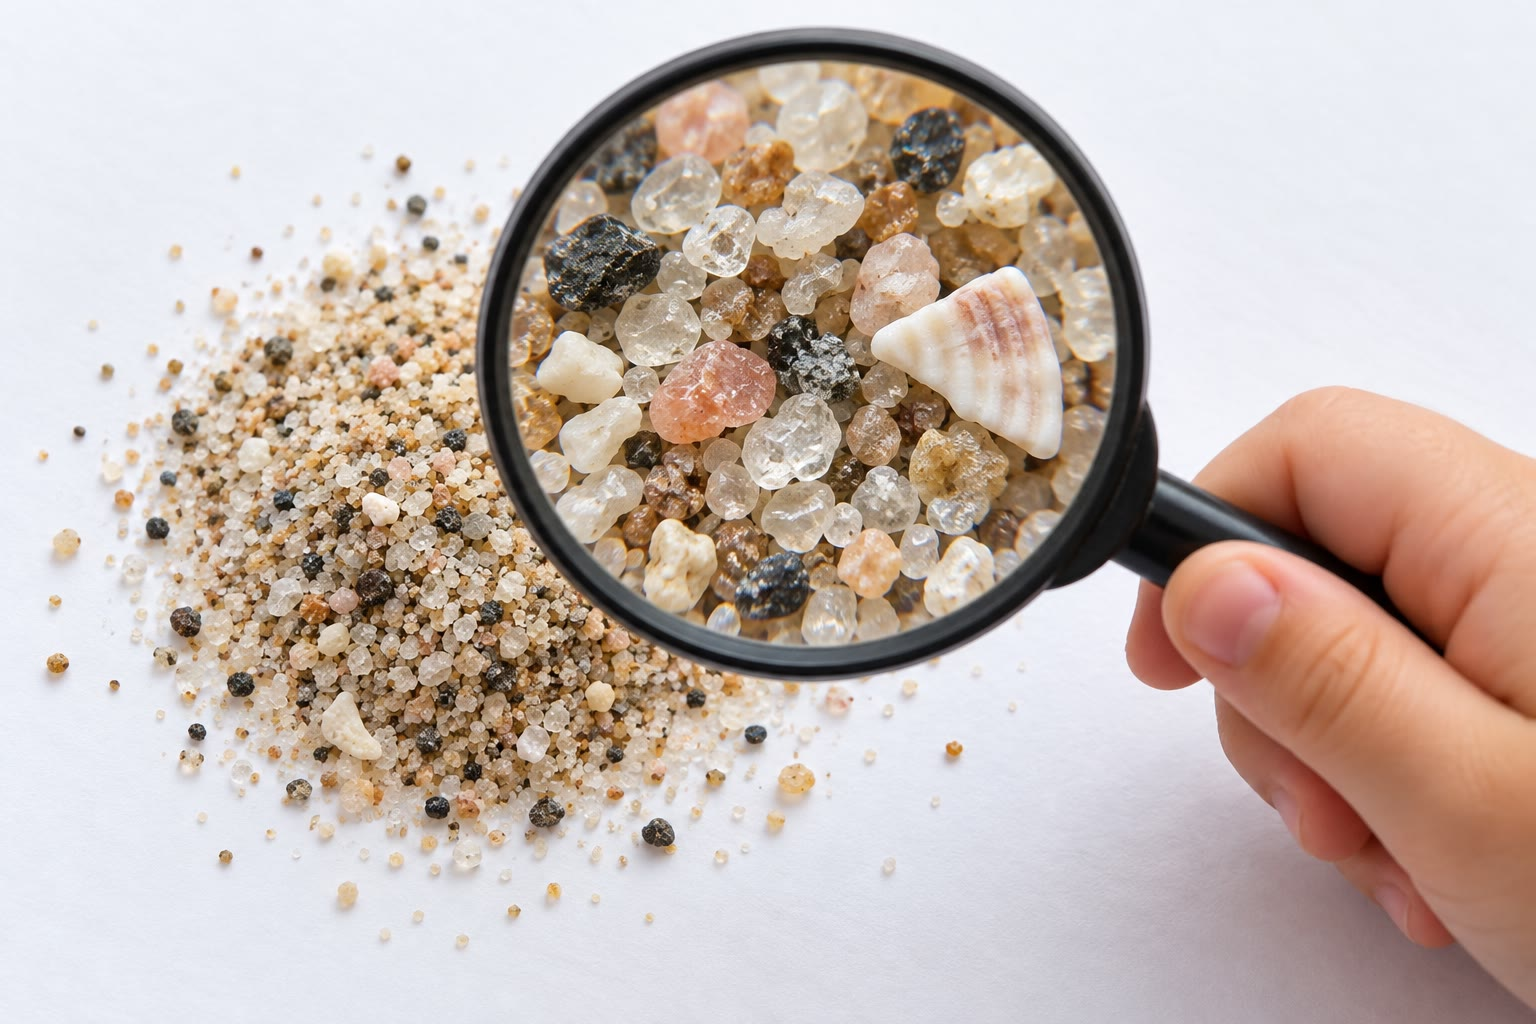
\includegraphics[width=0.55\linewidth]{images/book1/ai/g3-sand-magnifier.jpg}

{\small Beach \omterm{def:g3:stones-pebbles-sand:sand}{sand} seen through a magnifying glass: tiny grains of \omterm{def:g3:stones-pebbles-sand:rock}{rock}
and pieces of shell.}
\end{omfigure}

\begin{method}[Sorting broken rock by size]\label{met:g3:stones-pebbles-sand:sort}
To name a piece of broken \omterm{def:g3:stones-pebbles-sand:rock}{rock}, look at its size:
\begin{enumerate}
  \item if you cannot see the grains, even close up, it is \omterm{def:g3:stones-pebbles-sand:sand}{mud};
  \item if you can see each grain, but each one is smaller than 2
        millimetres (the thickness of a coin), it is \omterm{def:g3:stones-pebbles-sand:sand}{sand};
  \item if the pieces are bigger than that, but you can hold one in your
        hand, they are \omterm{def:g3:stones-pebbles-sand:pebble}{gravel} and \omterm{def:g3:stones-pebbles-sand:pebble}{pebbles};
  \item if a piece is too heavy to lift, it is a boulder.
\end{enumerate}
\end{method}

\begin{example}[Where do we find each size?]\label{ex:g3:stones-pebbles-sand:where}
Fast water can carry big stones; slow water drops them and carries only
small grains. So boulders and sharp stones lie in the steep \omterm{def:g1:landscapes-around-us:landform}{mountain}
streams; \omterm{def:g3:stones-pebbles-sand:pebble}{pebbles} and \omterm{def:g3:stones-pebbles-sand:pebble}{gravel} lie on the banks of the \omterm{def:g1:landscapes-around-us:water}{river} in the \omterm{def:g1:landscapes-around-us:landform}{valley};
\omterm{def:g3:stones-pebbles-sand:sand}{sand} gathers on beaches and in quiet bends of the \omterm{def:g1:landscapes-around-us:water}{river}; and \omterm{def:g3:stones-pebbles-sand:sand}{mud} settles
where the water is almost still, in ponds, \omterm{def:g1:landscapes-around-us:water}{lakes} and the mouths of \omterm{def:g1:landscapes-around-us:water}{rivers}.
\end{example}

\section{Hard rocks and soft rocks}

Not all \omterm{def:g3:stones-pebbles-sand:rock}{rocks} are equally hard. Some, like granite, are so hard that they
scratch glass and last for thousands of years in a wall. Others crumble in
the hand, like chalk, which leaves a white mark on a board. Some \omterm{def:g3:stones-pebbles-sand:rock}{rocks} are
made of grains that we can see; others are smooth and look all the same
from one side to the other.

\begin{example}[Three rocks compared]\label{ex:g3:stones-pebbles-sand:three}
\emph{Granite} is speckled with pink, white and black grains and is very
hard. \emph{Sandstone} is made of grains of \omterm{def:g3:stones-pebbles-sand:sand}{sand} stuck together; rubbed
with a finger, it sometimes lets a few grains go. \emph{Chalk} is white,
soft and powdery. You will learn in a later year how each of them was
formed.
\end{example}

\begin{omfigure}
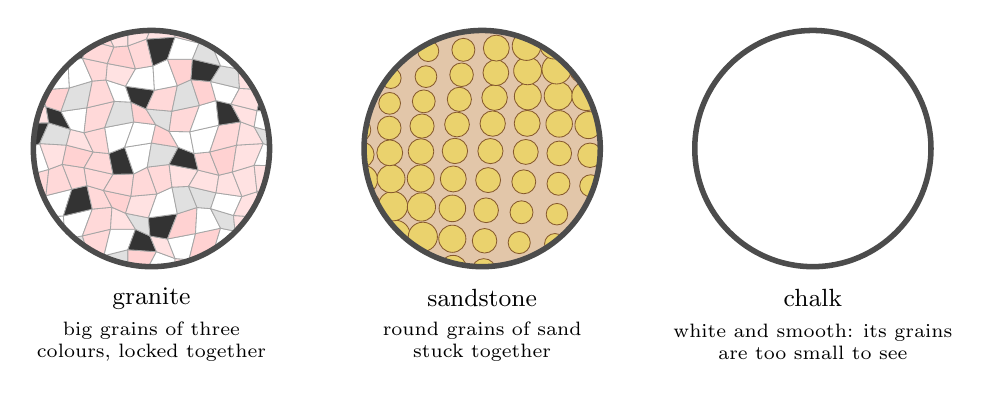
\begin{tikzpicture}[font=\small]
  % three stones seen through a magnifying glass (drawn, not to scale)
  % granite: interlocking grains of three colours
  \begin{scope}
    \clip (0,0) circle (1.5);
    % a jittered lattice: the cells tile the disk with no gap, like the
    % interlocking crystals of granite
    \foreach \i in {-6,...,5} \foreach \j in {-6,...,5} {
      \pgfmathtruncatemacro{\c}{mod(abs(37*\i+17*\j+\i*\j),7)}
      \ifcase\c \def\col{pink!70}\or\def\col{pink!45}\or\def\col{white}\or
        \def\col{black!12}\or\def\col{white}\or\def\col{black!80}\else\def\col{pink!60}\fi
      \fill[\col, draw=black!35, line width=0.3pt]
        ({0.27*\i+0.07*sin(90*\i+131*\j)},{0.27*\j+0.07*cos(77*\i+61*\j)}) --
        ({0.27*(\i+1)+0.07*sin(90*(\i+1)+131*\j)},{0.27*\j+0.07*cos(77*(\i+1)+61*\j)}) --
        ({0.27*(\i+1)+0.07*sin(90*(\i+1)+131*(\j+1))},{0.27*(\j+1)+0.07*cos(77*(\i+1)+61*(\j+1))}) --
        ({0.27*\i+0.07*sin(90*\i+131*(\j+1))},{0.27*(\j+1)+0.07*cos(77*\i+61*(\j+1))}) -- cycle;
    }
  \end{scope}
  \draw[black!70, line width=2pt] (0,0) circle (1.5);
  \node at (0,-1.9) {granite};
  \node[font=\scriptsize, align=center] at (0,-2.45) {big grains of three\\colours, locked together};
  % sandstone: rounded grains touching
  \begin{scope}[xshift=4.2cm]
    \clip (0,0) circle (1.5);
    \fill[brown!45] (-1.6,-1.6) rectangle (1.6,1.6);
    \foreach \x in {-1.5,-1.1,...,1.6} \foreach \y in {-1.5,-1.15,...,1.6}
      \fill[yellow!50!brown!70, draw=brown!70!black, line width=0.3pt]
        ({\x+0.08*sin(97*\x+61*\y)},{\y+0.07*cos(53*\x-89*\y)}) circle ({0.16+0.03*sin(71*\x*\y)});
  \end{scope}
  \draw[black!70, line width=2pt] (4.2,0) circle (1.5);
  \node at (4.2,-1.9) {sandstone};
  \node[font=\scriptsize, align=center] at (4.2,-2.45) {round grains of sand\\stuck together};
  % chalk: smooth, no grains to see
  \begin{scope}[xshift=8.4cm]
    \fill[white] (0,0) circle (1.5);
  \end{scope}
  \draw[black!70, line width=2pt] (8.4,0) circle (1.5);
  \node at (8.4,-1.9) {chalk};
  \node[font=\scriptsize, align=center] at (8.4,-2.45) {white and smooth: its grains\\are too small to see};
\end{tikzpicture}

{\small Three \omterm{def:g3:stones-pebbles-sand:rock}{rocks} seen through a magnifying glass (drawn). The grains of
granite and of sandstone can be seen; chalk looks the same everywhere.}
\label{fig:g3:stones-pebbles-sand:magnified}
\end{omfigure}

\begin{method}[Looking closely at a stone]\label{met:g3:stones-pebbles-sand:look}
To describe a stone, look at it and touch it, without breaking it:
\begin{enumerate}
  \item its colour, or its colours;
  \item its shape: sharp with corners, or round and smooth;
  \item its grains: can you see them? are they all the same, or of several
        colours?
  \item its feel: hard, or soft enough to leave a mark on paper?
\end{enumerate}
Write what you see in a table, one line for each stone.
\end{method}

\begin{example}[A table of three stones]\label{ex:g3:stones-pebbles-sand:table}
Mia describes three stones from a box at school.
\begin{center}\small
\begin{tabular}{llll}
\hline
Stone & Colour & Shape & Grains \\
\hline
A & pink, white and black & round & big, three colours \\
B & yellow-brown & sharp & small, all alike \\
C & white & sharp & none to see \\
\hline
\end{tabular}
\end{center}
Stone C also leaves a white mark on paper. From the example above, stone A
looks like granite, stone B like sandstone and stone C like chalk. Stone A
is round: water has rolled it for a long time.
\end{example}

\section{The stones we build with}

For thousands of years, people have built with the \omterm{def:g3:stones-pebbles-sand:rock}{rock} around them. In
the old villages of a region, the walls are often all of the same colour,
because they were built with the stone of the nearest \omterm{def:g1:landscapes-around-us:landform}{hill}.

\begin{definition}[Building stone]\label{def:g3:stones-pebbles-sand:building-stone}
A \emph{building stone}\index{building stone} is a \omterm{def:g3:stones-pebbles-sand:rock}{rock} that is cut or
shaped to build walls, roofs, steps, bridges or pavements.
\end{definition}

Each \omterm{def:g3:stones-pebbles-sand:rock}{rock} is good for something. Hard granite makes walls, steps and
kerbs that last for centuries. Some \omterm{def:g3:stones-pebbles-sand:rock}{rocks}, like slate, split into thin,
flat sheets: laid one over the other, they make roofs that keep the rain
out. Sandstone and limestone are soft enough to be cut into neat blocks.

\begin{omfigure}
\begin{minipage}[b]{0.49\linewidth}\centering
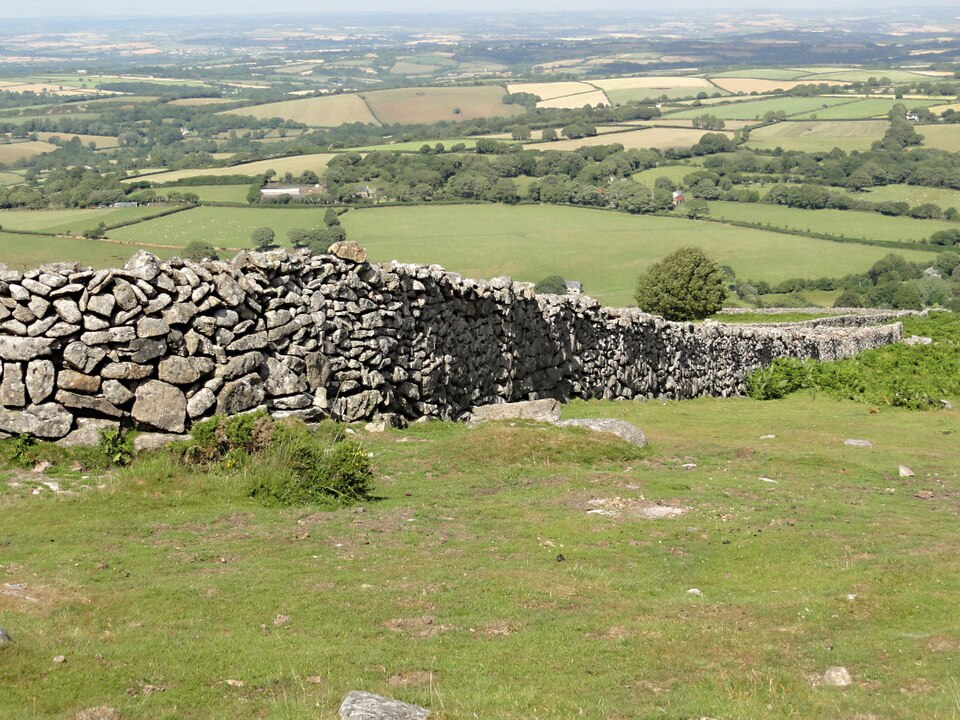
\includegraphics[width=\linewidth]{images/book1/g3-granite-wall.jpg}

{\small A wall of granite blocks, built without mortar. Photograph: Tony
Atkin, Geograph (CC BY-SA 2.0).}
\end{minipage}\hfill
\begin{minipage}[b]{0.49\linewidth}\centering
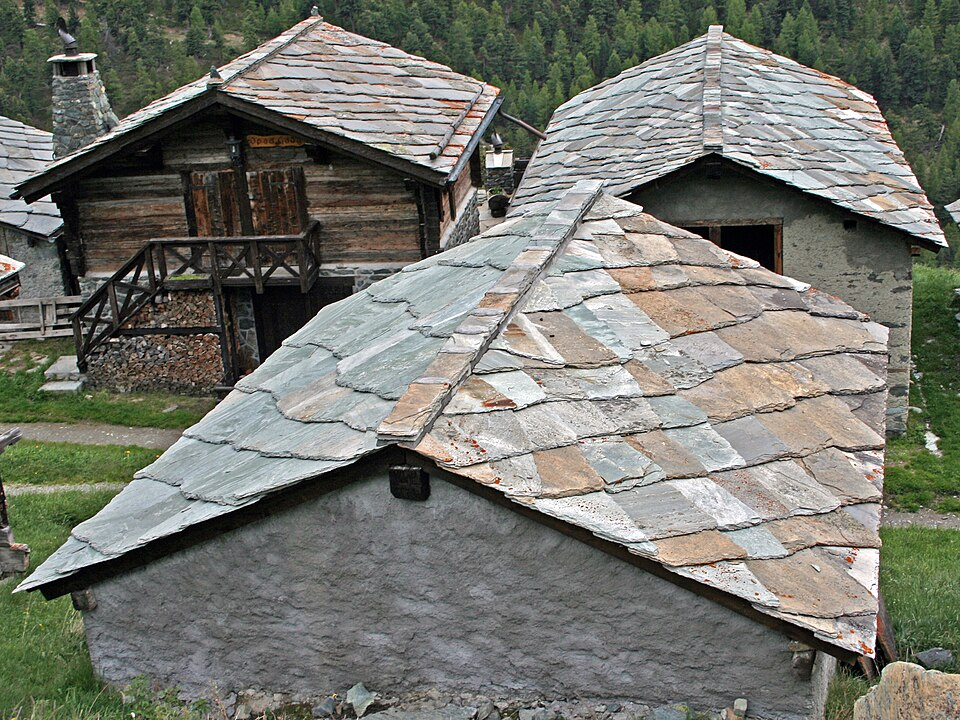
\includegraphics[width=\linewidth]{images/book1/g3-slate-roof.jpg}

{\small Roofs of thin, flat stone slabs in a \omterm{def:g1:landscapes-around-us:landform}{mountain} village of
Switzerland. Photograph: Michael C. Rygel (CC BY-SA 3.0).}
\end{minipage}
\end{omfigure}

\begin{omfigure}
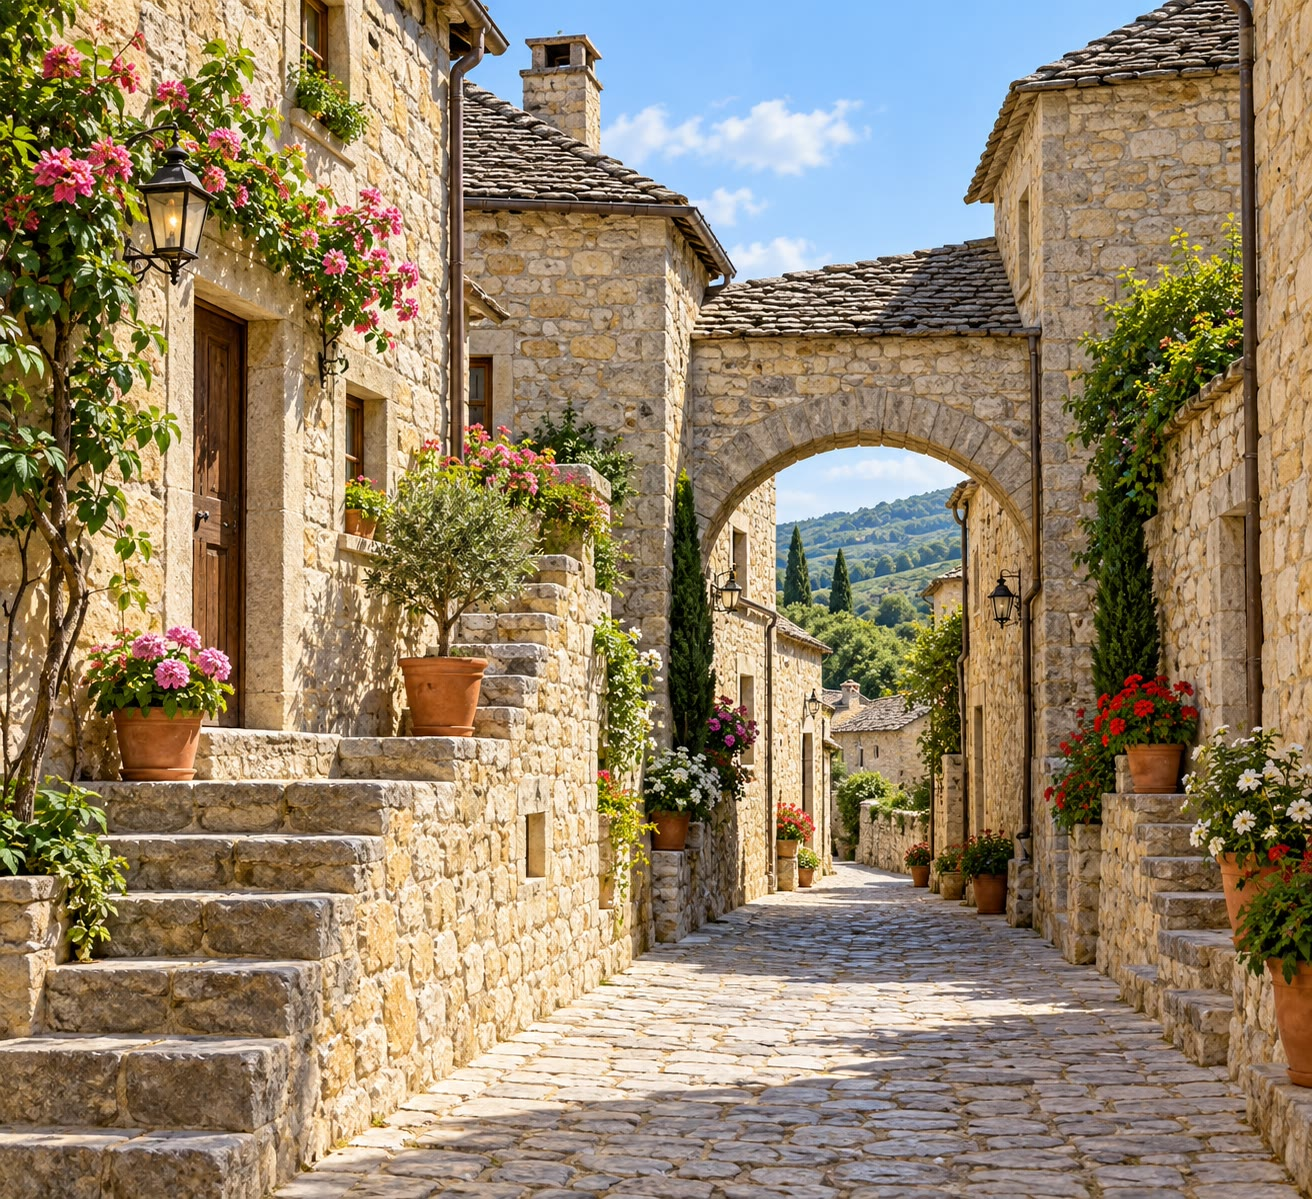
\includegraphics[width=0.6\linewidth]{images/book1/ai/g3-stone-village.jpg}

{\small An old village built entirely with the stone of the \omterm{def:g1:landscapes-around-us:landform}{hill} nearby.}
\end{omfigure}

Today we also build with bricks, concrete and glass. But a brick is made
of baked clay, concrete is made of \omterm{def:g3:stones-pebbles-sand:sand}{sand}, \omterm{def:g3:stones-pebbles-sand:pebble}{gravel} and cement, and glass is
made from \omterm{def:g3:stones-pebbles-sand:sand}{sand}: all of them come from the \omterm{def:g3:stones-pebbles-sand:rock}{rocks} of the Earth too.

\section{Exercises}

\begin{exercise}[$\star$]\label{exo:g3:stones-pebbles-sand:1}
What is the \omterm{def:g3:stones-pebbles-sand:rock}{bedrock}? Where can we see it without digging?
\end{exercise}

\begin{exercise}[$\star$]\label{exo:g3:stones-pebbles-sand:2}
Put in order of size, from the smallest to the biggest: \omterm{def:g3:stones-pebbles-sand:pebble}{pebble}, \omterm{def:g3:stones-pebbles-sand:sand}{mud},
boulder, \omterm{def:g3:stones-pebbles-sand:sand}{sand}.
\end{exercise}

\begin{exercise}[$\star$]\label{exo:g3:stones-pebbles-sand:3}
A grain is 1 millimetre across. Is it \omterm{def:g3:stones-pebbles-sand:sand}{sand} or \omterm{def:g3:stones-pebbles-sand:pebble}{gravel}? Another grain is
3 millimetres across: \omterm{def:g3:stones-pebbles-sand:sand}{sand} or \omterm{def:g3:stones-pebbles-sand:pebble}{gravel}?
\end{exercise}

\begin{exercise}[$\star$]\label{exo:g3:stones-pebbles-sand:4}
Natural or made by people? A \omterm{def:g3:stones-pebbles-sand:pebble}{pebble}; a brick; a block of granite; a sheet
of glass; \omterm{def:g3:stones-pebbles-sand:sand}{sand} on a beach.
\end{exercise}

\begin{exercise}[$\star$]\label{exo:g3:stones-pebbles-sand:5}
Why does a \omterm{def:g3:stones-pebbles-sand:pebble}{pebble} from a \omterm{def:g1:landscapes-around-us:water}{river} have no sharp corners?
\end{exercise}

\begin{exercise}[$\star$]\label{exo:g3:stones-pebbles-sand:6}
Name two \omterm{def:g3:stones-pebbles-sand:building-stone}{building stones} and say what each is used for in the photographs
of this chapter.
\end{exercise}

\begin{exercise}[$\star\star$]\label{exo:g3:stones-pebbles-sand:7}
Tom finds two stones of the same \omterm{def:g3:stones-pebbles-sand:rock}{rock}: one is sharp, the other is round.
Which one has travelled farther? Explain.
\end{exercise}

\begin{exercise}[$\star\star$]\label{exo:g3:stones-pebbles-sand:8}
On the grain-size drawing, how many centimetres long is the biggest \omterm{def:g3:stones-pebbles-sand:pebble}{pebble}?
How many \omterm{def:g3:stones-pebbles-sand:sand}{sand} grains of 2 millimetres would fit side by side along 1
centimetre?
\end{exercise}

\begin{exercise}[$\star\star$]\label{exo:g3:stones-pebbles-sand:9}
Where would you expect to find \omterm{def:g3:stones-pebbles-sand:sand}{mud}: in a fast \omterm{def:g1:landscapes-around-us:landform}{mountain} stream or in a
quiet pond? Why?
\end{exercise}

\begin{exercise}[$\star\star$]\label{exo:g3:stones-pebbles-sand:10}
Bricks, concrete and glass are made by people. Why can we still say that
they come from the \omterm{def:g3:stones-pebbles-sand:rock}{rocks} of the Earth?
\end{exercise}
